% Created 2020-10-25 Sun 18:51
% Intended LaTeX compiler: pdflatex
\documentclass[12pt,titlepage]{article}
\usepackage[utf8]{inputenc}
\usepackage[T1]{fontenc}
\usepackage{graphicx}
\usepackage{grffile}
\usepackage{longtable}
\usepackage{wrapfig}
\usepackage{rotating}
\usepackage[normalem]{ulem}
\usepackage{amsmath}
\usepackage{textcomp}
\usepackage{amssymb}
\usepackage{capt-of}
\usepackage{hyperref}
\usepackage[natbib=true]{biblatex} \DeclareFieldFormat{apacase}{#1} \addbibresource{./refs.bib}
\usepackage{parskip}
\usepackage[T1]{fontenc}
\usepackage{setspace}
\usepackage[english]{babel}
\usepackage[hyperref,x11names]{xcolor}
\usepackage[colorlinks=true,linkcolor=SteelBlue4,urlcolor=Firebrick4]{hyperref}
\author{Nandaja Varma Nandakumar}
\date{\textit{<2020-10-24 Sat>}}
\title{Stateful FaaS}
\hypersetup{
 pdfauthor={Nandaja Varma Nandakumar},
 pdftitle={Stateful FaaS},
 pdfkeywords={},
 pdfsubject={},
 pdfcreator={Emacs 27.1 (Org mode 9.3.7)}, 
 pdflang={English}}
\begin{document}

\maketitle
\begin{abstract}
Serverless Computing is an up and coming platform as a service offering 
where the cloud provider manages and allocates
resources needed to keep the application running. This lets the developer focus on the application development
and not on server maintenance. Alongside off loading the provisioning and
maintenance of the server, Serverless computing also reduces resource waste
by scaling up and down the allocation depending on the load and the
configurations. The users only pay for the resources that were used by the
application thereby saving huge operational cost on their infrastructure
hosting.

Although Serverless might sounds like the holy grail of application hosting, the 
current state of art technology fall short in several places to meet the industrial
requirements. Data intensive applications, streaming applications, and
distributed computing are some of the fields that could be benefited heavily by
implementation on Serverless platforms in terms of ease of development,
efficiency and cost. But all the existing platforms offer very
poor performance in these fields and works mostly via workarounds and n number
of third party tools.

This thesis analyses the Serverless paradigm in depth,
pointing out the reasons for this reduced adaptability. To solve these issues, we propose a lightweight
extension to an existing Open Source Serverless platform, OpenFaaS, by provide
flexibility, scalability and adaptability, while making sure not to violate the notion
of functions. Our implementation tries to reduce the operational gap between the
industrial applications and theoretical ideas produced by researches in the
academia in the past few years.
This thesis also offers a deep study of the full potential and limitations of
Serverless thereby making it clear to the reader why more innovations are
necessary in this field.

\end{abstract}

\setcounter{tocdepth}{4}
\tableofcontents


\section{Introduction}
\label{sec:org48b6b45}

Serverless can easily be considered as the new generation of platform as a
service. It can be thought of as an infrastructure where the programmer send
their application as functions in a predefined format, in a supported
programming language as documented by the provider. This function get hosted at
a certain endpoint which can be triggered with certain events supported by the
platform. In short, instead of having continuously running servers, functions operate as
event handlers and when the functions execute, the equivalent CPU usage is paid
for by the user. This has huge economical and architectural implications that is
still waiting to be explored in its full power. While the developers worry about
the logic of handling the requests/events, the infrastructure provider takes
care of receiving the request, responding to them, capacity planning, task
scheduling, and operational monitoring\cite{gotoconf}.

In the current industrial applications, data intensiveness of the applications are increasing
day by day paving way to adopt several resource heavy tools to do stream
processing, distributed processing etc. More than often CPU and memory loads in
these machines tent to vary a lot and rather than having a dedicated server to accommodate the whole range
of requirements, it makes perfect sense to convert it into a Serverless workload
thereby saving up on operational cost, resource waste, and ease of development.
Having said that, the current commercial offerings of Serverless do not work
very great with such workloads.

This is mostly due to the sheer
nature of the serverless paradigm of being completely stateless, thereby forcing
the developers to use external block storages for data store and communication.
In this thesis, we try to extend Serverless to leverage its full potential by
introducing an efficient form of state thereby providing flexibility, scalability and
adaptibility at the same time not violating the notion of functions in these platforms.
We will be extending an Open Source serverless platform called OpenFaaS
considering its simplistic and expandable architecture.

Currently most of the commercial serverless offerings are closed source
and vendor locked in to their respective platforms by cloud providers. But in the
past couple of years the field has gotten a lot of traction in the academia and
a lot of Open Source alternatives are being widely adopted. This being the case, a lot
of these works hasn't been properly applied in the industry, some because of
the absense of proper integrations with the industry standard tools, and some
because of the operational gap between the theoretical ideas and the
practicality or usability in the field. This thesis tries to reduce that
gap by proposing a very secure and multi-tenant implementation of a
state-ful Serverless setup which can be easily used for production quality
applications. A focus on the possibility to monitor the application performance
and usage provides a possibility to do fine grained billing of the resources and thereby
contributing to the easy adaptability of our extension.

Using our proposed Serverless setup, we try to efficiently run a
Extract-Transfer-Load(ETL) workload on streaming data. ETL basically is a pipeline that involves receiving data
from source, cleaning and transforming it, and loading it to a sink. We will
split the whole operation into multiple functions as per the Serverless notion
and have them communicate data and state internally to complete the pipeline
thereby reducing the latency and external bottlenecks.

This document describes more on Serverless paradigm, the shortcomings of it, the
ones we are trying to solve, our solution and evaluation. It is split into
several sections as follows:

In Section 2, we go a bit in depth to understand the history of cloud
infrastructure and the technological innovations that led to Serverless
paradigm. We also look in detail at the characteristics and nature of
Serverless. We look at some commercial Serverless offerings and understand how
in the programming world Serverless has influenced even in the way of developing.
We will also see what limitations it holds at its current state of evolution and
on solving which issue are we particularly interested in, in the scope of this
thesis.

In Section 4, we look at the current state of research in the field of
Serverless technologies and some related works.

In Section 3, We present the proposed solution for our Serverless setup going
into detail about how certain unacceptable limitations can be overcome.

In Section 4, the implementation of the system including the architecture and
the tools used is presented.

In Section 5, we go on with the evaluation of our system as opposed to standard
Serverless workloads.

We move on to Section 6 to understand the limitations of our proposed system.

In Section 7, the future work that can be done in this direction is laid out
before the reader.

\section{Background and Motivation}
\label{sec:org8154f99}
The term serverless have been vaguely thrown around the domain of cloud
infrastructure in the past decade as the breakthrough resource(and hence money)
saving tool that lets the developers focus on application logic rather than the
deployment and server maintenance. Having said that, it is often hard to define
what exactly serverless is since the service offering tend to change based on
the cloud provider and the interpretations of the users. It is fair to say that
serverless is a huge leap in the direction of using computational power as a
resource which can be paid for as per the usage.
Although the terminology is irrelevant, we will be focusing on the serverless
offering called Function-as-a-Service(FaaS) where the cloud providers offer a
platform to which we can upload our application code to(complying to the API
rules) and get uninterrupted service of the same at an endpoint irrespective of
the traffic or data load. Paying only for what resources has been used adds to
the attraction of the domain.
In this section, we will understand more about this technology, the
popular commercial offerings the same, and its limitations and the current state
of research. 
We will also analyze the popular data processing and streaming pipelines in the
industries these days and why serverless computing fall short in being the right
tool of development and deployment here.
\subsection{Evolution of cloud resource management}
\label{sec:org71894e9}
In the past 3 decades, software deployments and infrastructure management has
seen a lot of innovation and evolution. Before diving into the current
industrial standards, it is important to understand the evolutions in this field
to get a better grasp on the technological innovations that bought this about.


\subsubsection{Dedicated servers}
\label{sec:org2b33ece}
Even as recent as 15 years ago this was the industry standard for deployments. Dedicated servers
are physical machines. The general practice was to have server racks on the premise
of the company which are maintained by system administrators and all your
software is
hosted there. Although this method offers advanced security and high
availability, it is often common that a lot of physical resources were
underutilized and each resource was for single client. Not to mention the
environmental impact of the reserved heavy hardware which leaves a heavy carbon
footprint and e-wastes.


\subsubsection{Dedicated virtual machines(BaaS)}
\label{sec:org448a8dc}
Virtualization technology changed the face of software infrastructure by decoupling
applications from the underlying hardware. Virtualized servers are not physical
machines, they are a software construct. Virtual servers run on dedicated
servers, the resources of which are divided between several virtual servers.
To get slightly technical, virtualization usually involves installing a virtualization software(Hypervisor) on an
existing operating system and then having multiple operating systems on it,
sharing all the resources of the underlying operating system, yet providing
great security and isolation.

\begin{figure}[!h]
    \caption{My caption}
    \centering
    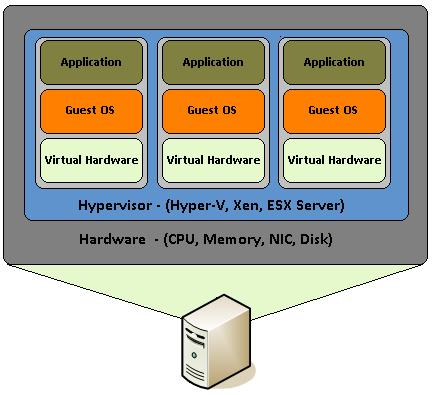
\includegraphics[width=80mm]{./thesis_images/virtual_machines.JPG}
    \label{fig:testing the label}
\end{figure}


Although applications in hosted on the virtual machine suffers from a heavy
input/output and network overload because of the added layer of indirection,
this technology reduces the resource waste to a great extend. The enterprises could share their hardware into
multiple virtual machines and have different hosting and computation in each of
the them. System administrators started splitting up their bare metal resources
among multiple Virtual Private Servers(VPS) by the help of virtualization
software. Each VPS would give you the feeling
of having a real system although it is a virtualized system which is sharing the
resources with other VPSs. This reduced a lot the amount of work and energy spent on
maintaining server racks along with the terrible underutilization of resources.

More and more companies started adapting this technology and in early 2006
Amazon Web Services(AWS) re-launched themselves as a platform that offers
computing and storage space to developers and enterprises on an on-demand basis
revolutionizing how companies were designing their system architecture. Soon
after Google and Microsoft followed suit with their cloud infrastructure
platforms offering similar services. All these providers function by maintaining
huge, dedicated server farms across the globe to provide the necessary resources
to the customers.

These kind of services, generally called as Infrastructure as a Service(IaaS) or
Platform as a Service(PaaS), went through a
series of changes during the past decade. On-demand compute instances to
completely managed deployment services(eg: Google App Engine), Pay per use block
storages(AWS S3) to fully managed dedicated relational databases(Google Cloud
SQL, AWS RDS, etc.) a lot of really efficient and interesting services started
to be available for the developers disposition. The billing scheme of these
services also started to be quite flexible even allowing a per second billing
plan in the past couple of years by Google.

It is also worth noting that with the advent of virtualization, the job profiles
in several companies shifted from having a system administrator role to 
having profiles called DevOps(development and
operations) who are application developers focusing on the provisioning of the
virtual machines to deploy their applications. Although IaaS solved a lot of
hassle around infrastructure provisioning, the systems and load of the
applications still remained independent. Applications always had dedicated virtual machines
even if the load/traffic to and fro the application is not constant. This meant that a
lot of resources were still being wasted.

\paragraph{Linux Containers}
\label{sec:org08c20fa}
A game changer in the world of virtualization was containerization. Containers
are yet another packaged computing environment that combine various IT
components and isolate them from the rest of the system just like a virtual
machine would. It was developed to solve a lot of problems with virtual
machines. The purpose of the containers is to encapsulate an application and its dependencies within its own environment. This allows them to run in isolation while they are using the same system resources and the same operating system. Since the resources are not wasted on running separate operating systems tasks, containerization allows for a much quicker, lightweight deployment of applications. Each container image could be only a few megabytes in size, making it easier to share, migrate, and move.
[containers]cite Even though Linux Containers
have existed for a very long time, in the past decade, containers were made a
lot more approachable and adaptable as a
technology by the advent of communities like Docker and rkt.  the user space

The light weight of the containers
made it the ideal candidate for running applications. What makes container based deployments special
as opposed to the ones deployed directly on the host is the consistency of the environment. The application
execution environment can be recreated and ported from one system to another without affecting the functionality
of the application or having to reinstall the whole binary dependencies on the new machine. Reproducability of the
production environment even in the local exactly, meant that the development/testing cycle became much more efficient.
The isolated package of the application, enveloped as a container image, is
agnostic of the operating system it runs on opening new possibilities for the
deployment. One could also limit and fine tune the resources used by a running
containers giving a lot more control over the application.

\paragraph{Autoscaling}
\label{sec:orgc98dbdb}
The ease in which one can limit the resources and tweak the runtime parameters externally contributed heavily
to the service offering called autoscaling which basically meant resources for an
application runtime were added or removed as per the usage. All the commercial
cloud providers started offering the aforementioned service in different
flavors. Autoscaling on EC2 or Google Compute, AWS Fargate, etc. are some examples.

In the past two years, innovations have taken a leap in the field of isolation
environments, introducing solutions like AWS Firecracker, Cloudflare workers,
etc. to the community. These solutions aim at mitigating the shortcomings of
Containers which we will discuss in Section 2.2.4

\subsubsection{Serverless}
\label{sec:org7786448}
Like mentioned earlier, in the past two years the terms Serverless and Function-as-a-Service are quite
often used interchangeably. In terms of the resource reservation, Serverless can
be considered as a platform as a service solution that scales. Your application
will always have enough and only enough resources dedicated to it. It will scale
up and down based on the load and traffic and the developer only pays for the usage.
This paradigm of autoscaling has been hence applied even to database storage
solutions by major cloud providers such that even the block storage is allocated
based on usage and there will be a burst of reservation as soon as a certain
limit is reached.
The pioneers of this technology can be considered as the proprietary service
Lambda by Amazon Web Services[CITE]. Several other cloud providers followed suit
with similar platforms specific to their infrastructure.
The nature of serverless makes it attractive for both developers and the cloud
providers since in the case of former, it means paying much less and in case of
the latter, it means they can easily provide shared tenant resource allocation
units.

We will dive more into the properties and nature of the solution
Function-as-a-Service(FaaS) in the following session. 

\subsection{FaaS}
\label{sec:org822f92d}
So far, we have covered the infrastructure management style of FaaS or
Serverless in general. Let us get a bit in detail into the specifics of the
hosting platform that provides the FaaS functionality.

Most FaaS platforms being closed source, provides the client API for developers
to supply a package including their code and dependencies to. Most platforms
supports a limited set of programming language runtime although it is usually
possible to do workarounds to deploy custom runtime. Behind the screen,
the platform containerizes the application and deploy it so as to get triggered
via pre-defined hooks specified by the developer. The infrastructure also provides endpoints or
interfaces to specify the maximum and minimum CPU and memory allocated for the
application, the maximum timeout for the application(although there is a
hard bound on this imposed by the infrastructure provider usually). To
understand the flow of FaaS workloads, it is important to be aware of the
following properties of the platform.

\subsubsection{Properties of FaaS}
\label{sec:orga963f6b}
\paragraph{Statelessness}
\label{sec:org7a847da}
\begin{itemize}
\item the functions execute, they just take in data, process and output.
\end{itemize}
\paragraph{Triggers}
\label{sec:org48a8be1}
\paragraph{Parallelism}
\label{sec:orgf6d4226}
\paragraph{Developer friendliness}
\label{sec:org80fcbb0}
\subparagraph{Dependency management}
\label{sec:orgba2065a}
\subparagraph{Debugging and testing}
\label{sec:orgb425ffd}
\subparagraph{Deployment}
\label{sec:orgdfd3c44}
\subparagraph{Logging and monitoring}
\label{sec:org5fcd3ec}
\paragraph{Billing}
\label{sec:org02241b2}

\subsubsection{How programming models are getting affected by this}
\label{sec:orgc340539}
\paragraph{Faas + Microservices}
\label{sec:orgd119a1f}
\paragraph{Statelessness a.k.a Functional programming model}
\label{sec:org04c77b9}
\subsubsection{Popular commercial offerings}
\label{sec:org1049e50}
\paragraph{AWS Lambda}
\label{sec:org34ea423}
\paragraph{Google cloud functions}
\label{sec:orgdd3eea0}
\paragraph{Azure functions}
\label{sec:orged5451e}
\subsubsection{Where serverless computing fall short}
\label{sec:org089ed60}
Although serverless computing might sound like the silver bullet of the
deployment solutions, it is a field that is still being rapidly grown and
researched on. There are several staggering shortcomings for this technology
that makes it unsuitable for certain applications. The current offering have the
following noticeable limitations.
\paragraph{Lack of state}
\label{sec:org009c8a2}
The serverless/auto-scaling paradigm generally push for a development style
involving no state to make the infrastructure simple encouraging a functional
style of development. Although this can contribute to easily scalable and
parallelisable applications, it often limits the technology from being adapted
in applications that are data intensive and/or requires faster response times.
The fact that serverless functions don't store any intermediate state requires
the application developers to use a block storage to store the data and state
after the execution. This basically means communication via slow storage and
adds a lot to the latency. This discourages the use of serverless in distributed
computing which is actually a domain that needs very fine grained communication
between the functions and usually a lot of resources are wastefully dedicated to
ensure high availability.
\subparagraph{Coordination issues among functions}
\label{sec:orgbbbd43c}
\begin{enumerate}
\item ETL
\label{sec:org7ea15d6}
\item Distributed Computing
\label{sec:org741f305}
\end{enumerate}
\paragraph{Latency IO}
\label{sec:orgbbdf0a2}
data shipping vs function shipping
\paragraph{Vendor lock in}
\label{sec:orgccc7ba8}
It is no secret that the most widely used FaaS/serverless offerings are the ones by
proprietary cloud providers where they hand twist the developers into complying
to their programming environment and runtime thereby forcing devs to use their
technologies. What such practices contribute to is limited innovations and
development around the paradigm of Function as a service itself and people
re-inventing the wheel by creating custom made code and hack to fit each of
these provider runtimes.
\paragraph{Fixed timeouts}
\label{sec:org2da74b9}
\paragraph{Latencies}
\label{sec:org7c6c6c2}
\subparagraph{Start up time}
\label{sec:org4e6ae1c}
\subparagraph{Library loading time}
\label{sec:org20897cd}
\paragraph{Security issues in a multitenant environment}
\label{sec:org98e68c8}
\subparagraph{Function caches}
\label{sec:orge3c00b8}
\subparagraph{Containers introducing bugs}
\label{sec:org2588392}
code shopping data shipping
between functions adding to the latency, cost, and inconvenience. From a
technical point of you this can be described as serverless architecture being a
data shipping one rather than a code or function shipping one. Meaning, rather
that moving the code to the platform where the data is and executing it there,
serverless follows the paradigm where  
\subsection{Stream Processing/ETLs}
\label{sec:org3e6b8d5}
\subsection{Problem statement}
\label{sec:org86daac4}
\subsubsection{With the current state of development in the field of streaming and other data}
\label{sec:orgb334d3f}
intensive applications, a serverless/FaaS platform could really help save
resources and hence operational cost of applications.
\subsubsection{Having a platform that can take care of the resource provisioning for you, when}
\label{sec:orgb909c28}
you can focus on the program logic and the data engineering side, helps a lot of
domain specific engineers test out and deploy their applications easily.
\subsubsection{A lot of the existing platforms already do it, but most of these solutions available}
\label{sec:org7259571}
commercially are extremely vendor locked in. The limitations are set for you by
the cloud providers and is often very difficult to fiddle with it or to extend
the system so as to support an extra runtime etc.
\subsubsection{Along with this, the way current FaaS offerings deal with function compositions}
\label{sec:org1b9d92b}
and parallelism are extremely clumsy and almost always explicit. While this lets
the providers have a very generic way of dealing with the platform and holds to
the one way to code them all paradigm, the gateways often tend to be a
bottleneck. Also the data transfer between functions always depend on a storage
based off of Block IO which contribute to the latency immensely.
\subsubsection{I propose a platform based off of an OpenSource FaaS infrastructure that can be}
\label{sec:orgf59ec19}
maintained by the companies which can offer a multitenant and completely elastic
platform to deploy their data intensive and high throughput applications on.
When I say completely elastic, it means that the intermediate datastore tend to
be ephermeral and that scales to based on the usage incurred by the system and
offers fine grained usage monitoring and billing if need be. Alongside,
providing an easy to use API that lets one compose functions 




\section{Related work}
\label{sec:orgf7add76}
\section{Proposed Solution}
\label{sec:org60892b8}
\subsection{Introducing autoscaling ephermeral storage to ETLs.}
\label{sec:org4b00788}
\subsubsection{Describe pocket and the way it works.}
\label{sec:org780d159}
\subsection{Function composition to pass and retrieve the data in the middle stages}
\label{sec:orge07dbfb}
\subsubsection{branching and jumping}
\label{sec:org0713569}
\subsection{Multitenancy support by namespaces}
\label{sec:orgc705e44}
\subsection{Tracking the usage fine grained and billing data accordingly}
\label{sec:org4f92a19}
\section{Implementation}
\label{sec:org82227af}
\subsection{Architecture}
\label{sec:orgaf976c7}
\subsection{Tools}
\label{sec:orgf69c98f}
\subsubsection{OpenFaaS}
\label{sec:org5351e96}
\subsubsection{Pocket}
\label{sec:orgb25dc72}
\subsubsection{Kubernetes}
\label{sec:org242b5f4}
\subsubsection{FaaS-flow}
\label{sec:org4952c37}
\subsubsection{Prometheus}
\label{sec:orge1fa1d1}
\section{Evaluation}
\label{sec:orgc39e987}
\section{Future work}
\label{sec:org8795e6a}
\section{Conclusion}
\label{sec:orgfc4859a}


:UNNUMBERED: t
\end{document}
